\documentclass[12pt]{book}

\usepackage{amsmath}
\usepackage{hyperref}
\usepackage{color}
\usepackage{enumerate}
\usepackage{fancyhdr}
\setlength{\headheight}{30pt}


\setlength{\oddsidemargin}{0cm}
\setlength{\evensidemargin}{0cm}
\setlength{\textwidth}{6.5in}
\setlength{\topmargin}{-2.2cm}
\setlength{\textheight}{9.3in}
 \pagestyle{plain}
\pagestyle{fancyplain}
\fancyhf{}
\lhead{ \fancyplain{}{ABC Player} }
\rhead{ \fancyplain{}{Andrei Ivanov, Olga Shestopalova, Zeke Schmois} }
\rfoot{ \fancyplain{}{\thepage} }

\renewcommand{\arraystretch}{1.5}	
\newcommand{\Ri}{\ \Rightarrow\ }
\newcommand{\Le}{\ \Leftarrow\ }
\newcommand{\Lr}{\ \Leftrightarrow\ }
\newcommand{\ds}{\displaystyle}
\newcommand{\ts}{\textstyle}
\newcommand{\sst}{\scriptstyle}
\newcommand{\sss}{\scriptscriptstyle}
\newcommand{\q}{\quad}
\newcommand{\ap}{\alpha}
\newcommand{\ii}{\^{\i}n }
\newcommand{\si}{\c{s}i }
\newcommand{\oaf}{oricare ar fi }
\newcommand{\nn}{\mathbb{N}}
\newcommand{\ns}{\mathbb{N}^{*}}
\newcommand{\rr}{\mathbb{R}}
\newcommand{\rs}{\mathbb{R}^{*}}
\newcommand{\cc}{\mathbb{C}}
\newcommand{\zz}{\mathbb{Z}}
\newcommand{\zs}{\mathbb{Z}^{*}}
\newcommand{\qq}{\mathbb{Q}}
\newcommand{\qs}{\mathbb{Q}^{*}}
\newcommand{\g}{\mathbb{G}}
\newcommand{\di}{\displaystyle}
\newcommand{\ai}{astfel \^{\i}nc\^{a}t }
\newcommand{\la}{\lambda}
\newcommand{\s}{\sigma}
\newcommand{\ri}{\ \rightarrow\ }
\newcommand{\gr}{^{\circ}}
\usepackage{graphicx}


\begin{document}
%%%%%%%%%%%%%%%%%%%%%%%%%%%%%%%%%%%%
%%%%%%%%%%%%%%%%%%%%%%%%%%%%%%%%%%%%
%%%%%%%%%%%%%%%%%%%%%%%%%%%%%%%%%%%%
%%%%%%%%%%%%%-------1------%%%%%%%%%%%%%%%%%
%%%%%%%%%%%%%%%%%%%%%%%%%%%%%%%%%%%%
%%%%%%%%%%%%%%%%%%%%%%%%%%%%%%%%%%%%
%%%%%%%%%%%%%%%%%%%%%%%%%%%%%%%%%%%%
%%%%%%%%%%%%%%%%%%%%%%%%%%%%%%%%%%%%
\phantom{xxx}
\bigskip
\centerline{{\large \bf ABC Parser Project: Design Description }}
\bigskip\bigskip

\noindent {\textbf{Overview:}}

We represent an ABC parser for music files as a series of well-structured interfaces. When an ABC Music file is selected from the menu, it will be read and converted into a string, which will then be passed to the lexer to create tokens, which are then fed to the parser to walk the tree and create {\tt Music} objects, which then provide the necessary information to create and play the MIDI file created.

\noindent {\textbf{Revision Summary:}}

The lexer was changed to read duplet, triplet, and quadruplet parenthesis and digit as one token (so no quintuplets and up are allowed). The parser was changed to include a line rule that groups measures with lyrics to make adding lyrics to particular measures easier. It also was changed to include duplet, triplet, and quadruplet rules, also to make it easier to find and modify the notes associated with those.

Main was modified to include a pop up window to select the song to play.

\centerline{ 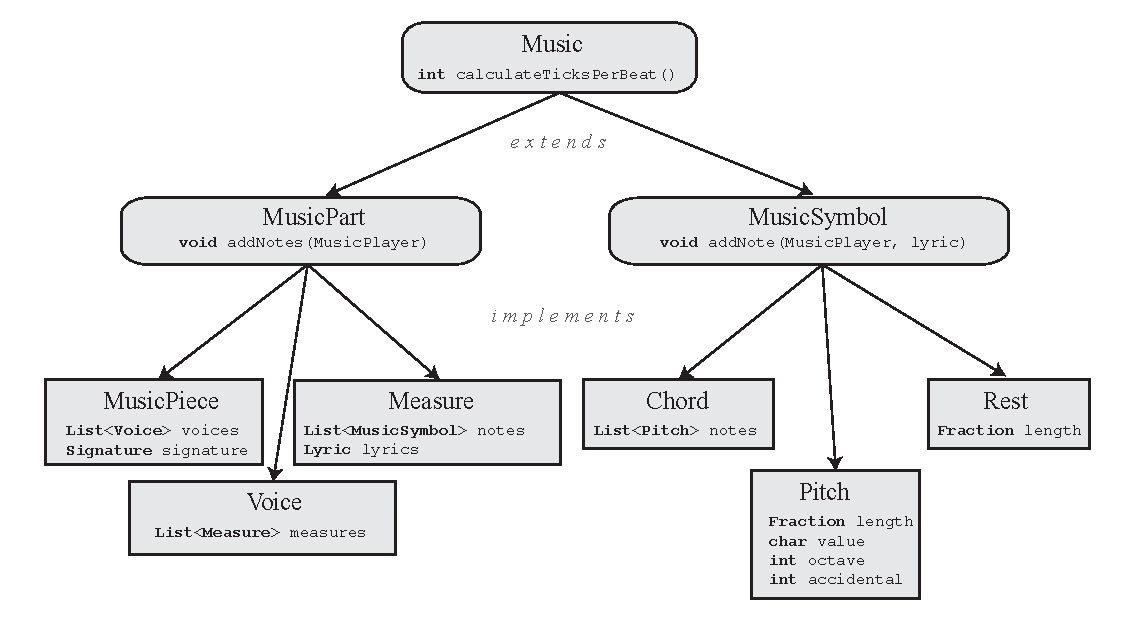
\includegraphics{Music.pdf}}

\noindent {\tt Music} is an interface that will represent our ADT. All {\tt Music} objects are immutable. It defines the following method

\begin{itemize} 

\item { \tt calculateTicksPerBeat} is an auxiliar method needed to determine the number of ticks per beat for the player such that any notelength can be represented as an integer number of ticks. The method is called recursively.
\end{itemize}

\medskip 

\noindent {\tt MusicPart} is an interface that extends {\tt Music} and represents either a {\tt MusicPiece} or {\tt Voice}.  It defines a method
\begin{itemize} 
\item { \tt addNotes} which takes an instance of  {\tt MusicPlayer} (described later) and adds to it all notes and lyrics found in the current {\tt MusicPart}  . It is called recursively.
\end{itemize}

\noindent and is implemented by the following classes:
\begin{itemize} 
\item { \tt MusicPiece} represents a final piece of music.   It has a {\tt signature} attribute which contains all the header information and {\tt List<Voice> voices} attribute which represents a list of different voices contained in this piece.
\item {\tt Voice}  represents a single voice in a piece of music. It has a {\tt List<Measure> measures } attribute which represents the sequence of measures the voice is made of.
\item {\tt Measure}  represents a single measure in a voice. It has a {\tt List<MusicSymbol>notes } attribute which represents the sequence of notes contained in the measure and a  {\tt List<Syllable> lyrics } attribute that represents the lyrics that accompain the measure.
\end{itemize}

\bigskip

\noindent {\tt MusicSymbol} is another interface that extends {\tt Music} and represents either a {\tt Pitch}, a {\tt Rest} or a {\tt Chord}. It defines a method
\begin{itemize} 
\item { \tt addNote} which takes an instance of  {\tt MusicPlayer} and a lyric corresponding to the current symbol and modifies the player by adding notes and lyric to it. 
\end{itemize}
\noindent and is implemented by classes:
\begin{itemize} 
\item { \tt Pitch} represents a single pitch. Its attribute {\tt length} is represented by a fraction  of the length of the default note. The attribute {\tt value} is a pitch A,B,C,...,G from the middle octave,  {\tt octave} represents the offset from the middle octave and  {\tt accidental} is 1 for sharp and -2 for flat. Using these conviniences,  a {\tt Pitch} from out ADT can be easily converted to the {\tt Pitch} object described in the {\tt sound} package.
\item { \tt Rest} represents a single rest and has an attribute {\tt length}  represented by a fraction of the length of the default note. 
\item {\tt Chord} represents a chord of several pitches and stores them in the {\tt List<Pitch>} attribute.
\end{itemize}

These three basic music symbols let us implement any "musical expression" defined in the 6.005 subset. Any other structures like tuplets, triplets, repeats, etc. are converted to these basic music symbols during the ParseTree walk.  

We also use an immutable class {\tt Signature} inside MusicPiece that has all header information stored in its attributes and a mutable class {\tt Lyric} which represents a list of lyrics used for each measure.

\bigskip
Another important class is a mutable {\tt MusicPlayer} which has two attributes 
\begin{itemize} 
\item { \tt player} that represents an instance of the {\tt SequencePlayer}. It collects the notes and lyrics of the song.
\item { \tt ticksPerBeat} which represents the number of ticks per beat in the {\tt player}
\item { \tt currentTick} which represents the current tick inside the player. It is used when the notes and lyrics are added consecutively to the player by the method {\tt addNote} to keep track of the position  where the notes need to be inserted. {\tt addNote} method increments it according to the length of the note.
\end{itemize}
It has the following methods:
\begin{itemize} 
\item { \tt addNote (int note,Faction length)} that takes a converted Midi note and inserts it in the {\tt player} at the {\tt currentTick} position.
\item { \tt addLyric (String Lyric)} that takes a syllable and adds it to the {\tt LyricListener} at the {\tt currentTicks} position.
\item { \tt addTime Fraction length)} increases the {\tt currentTick} by the length of the note.
\item { \tt resetTime() } resets the {\tt currentTicks} to 0. This is used when starting a new voice.
\item { \tt play() } plays the notes and lyrics added.
\end{itemize}


\centerline{{\large \bf Parsing }}

\begin{itemize}
\item {\bf Lexer}: The lexer is designed such that all of the header lines (ie. title, composer, etc) are each lexed as one token, as are all lyric and comment lines. Notes are lexed together with their modifiers (accidentals, octaves, duration) as one token. Duplet, triplet, and quadruplet parenthesis and digits are lexed as a single token (apart from their notes). Chord brackets are lexed separately from their notes. Pipes, repeats, and end of measure symbols are lexed as their own tokens. All whitespace except for newlines (/n/r) is skipped.

\item {\bf Parser}: The parser has rules for the whole musical piece, which is then broken into the header rules and the actual musical body rules. Each header line has its own rule, with title, number and key being mandatory. The musical body consists of either lines, voices, and/or comments. 

Lines are measures followed by a newline, optionally followed by a lyric. Measures are note elements optionally surrounded by repeats or pipes, but must end with either a repeat, an end of measure symbol, or a newline. 

A note element is a note, rest, chord, duplet, triplet, or quadruplet. Duplets, triplets, and quadruplets are the particular header token followed by 2, 3, or 4 notes or chords, respectively. A chord is a number of notes or rests enclosed in square brackets. Note, rest, and lyric have their own rules as well, which are just their respective lexer tokens.

\item {\bf Errors}: Errors in parsing and lexing result in an exception being thrown. (reportErrorsAsExceptions is invoked on both parser and lexer).

\item {\bf Listener}: While parsing the tree, we care about these events: exit note, exit rest, exit duplet, exit triplet, exit quadruplet, exit chord, enter measure, exit measure, enter line, exit line, exit lyric, enter voice, exit header, exit tune. Several stacks are present at once, for each kind of object.

When exiting the tune, voices and signature will be added to a MusicPiece object, which is then added to the stack.

When exiting a header, the information is extracted from the context, and defaults are added if necessary. A default voice is set if none are provided. The current voice is kept track of.

When entering a voice, the current voice is switched.

When entering a line, a new list of repeated ranges is created.

When exiting a line, lyrics are matched with their notes in their measure, and padded as necessary. Measure objects are created and added to the stack. If the measure index matches an index in the repeated range, that measure is added again (to the top of the stack). 

When entering and exiting a measure, repeats/n-th repeat/end of line symbols are searched for and the repeated range list is updated accordingly.

When exiting a lyric, the chunk of text will be sent to another lexer and parser, which will return a list of lists of syllables, which will be pushed to the stack.

When exiting a chord, the number of notes or rests inside is determined, then they are popped, and then added to a Chord object, which is then added to the stack (this object represents a list of notes, since they all start at the same time).

When exiting a duplet, triplet, or quadruplet, notes inside are popped, and their duration is modified accordingly, and the new notes are inserted back into stack.

When exiting a note or rest, we extract the needed information from the context and add a Pitch or Rest object to the stack. 


\item {\bf Tests}:
\begin{itemize}
\item Lexer: Test different inputs and make sure tokens are broken up correctly. 
Examples: Simple header only, extended header, header and body, lyrics, music that includes chords, tuplets, repeats, music that has comments, music with all different modifiers
\item Parser: Test different inputs and expect fully-formed MusicPiece objects to be returned. 
Examples: Just a Signature, Pitches, Rests, Chords, Lyrics, multiple Voices, repeated measures, all kinds of notes and modifiers
\item ADT tests: test the methods of our ADTs
Examples: equals, toString, hashCode, calculateTicksPerBeat, multiplyDuration, multiplyDuration, getLength, addNote, addNotes, etc.
\item Play: Testing the whole system, making sure that a file will be read in correctly, then lexed, parsed, and played.
Examples: pass in all of the sample\_abc files to be played, they contain the varying inputs that we want (simple measures, measures with comments, multiple voices, repeated sections, chords, tuplets, rests).
\end{itemize}

\end{itemize}

\newpage

\newpage
\centerline{{\large \bf Parsing Lyrics}}

\begin{itemize}
\item {\bf Lexer}: The lyrics lexer is designed to be simple and flexible and at the same time robust and capable of parsing everything deemed a good input. We start at the bottom token, LINESPACE. New line tokens are skipped because we have no special action to take when these are encountered. WHITESPACE follows and would normally also be skipped but because of the special WHITESPACE HYPHEN token, we must keep it in (this is explained with more detail in the parser rules). PIPEs are also unique tokens as they are used to separate measures. Then we have all the different symbols used to create different kind of syllables. Most importantly to note is that EXTENDERS and STARS can be one or more of the same while HYPHENs, DOUBHYPHENs, and UNION\_OPERs are composed of single characters. Finally is the WORD token which creates the most complex form of lyric possible, and is composed of all allowed, non-special characters in a lyric.

\item {\bf Parser}:
These rules define the structures used by the parser:
A well constructed lyric will be parsed as follows
\begin{itemize} 
\item lyric:
\begin{itemize}
\item can have multiple measures and any amount of trailing whitespace at the end
\end{itemize}
\item measure:
\begin{itemize}
\item can be an entire lyric if no PIPEs are found
\item can be empty or a cluster (the first word in the cluster determines the first token)
\item if it begins with a PIPE, it may have WHITESPACE*
\item if it ends with a PIPE, optional WHITESPACE* may be used to separate the last syllable
\end{itemize}
\item syllable:
\begin{itemize} 
\item can ONLY start with a WORD or a STARS
\item single syllable and single STARS can be considered a full cluster
\item no combination of WORD and STARS are allowed in the same syllable
\item WHITESPACE* is allowed at the end of every syllable
\item if starting with a WORD it must be followed by:
\begin{itemize}
\item a HYPHEN and\/or EXTENDERS
\item a WHITESPACE and HYPHEN and\/or EXTENDERS
\item a DOUBHYPHEN
\item a UNION\_OPER
\item EXTENDERS
\end{itemize}
\end{itemize}
\end{itemize}

\item Anything outside of these rules will be considered an incorrectly inputed
lyric and will throw an exception\/fail silently with an unexpected outcome

\item {\bf Errors}: Errors in parsing and lexing result in an exception being thrown. (reportErrorsAsExceptions is invoked on both parser and lexer).

\item {\bf Listener}: The lyrics listener is very simple as well. The lyrics object is composed of an ArrayList of ArrayLists of Strings, where each String is a ``syllable''. So, when entering a new Measure, we add an empty ArrayList to the main ArrayList. The only other event is exiting a Syllable. In this case, we consider every valid input and do a second ``parsing'' accordingly. This is actually the pretty-print that we implement for our frontend. It converts things like two-word syllables joined by ``~'' into two words joined by whitespaces.

The end product is an ArrayList<ArrayList<String>>, not null, and processed enough to use a literal toString() method to print to the user's console.

\item {\bf Tests}:
\begin{itemize}
\item Lexer:
\begin{itemize}
\item Tests the LyricsLexer, ensures tokens are what they should be. Tests all kinds of lyrics.

\item Testing space:

\begin{itemize} 
\item We assume valid inputs. We create tests which lex one token at a time. Once every token is tested for, we introduce multiple tokens in the same input stream. A stream with all tokens is the upperbound while a stream with one token is the lowerbound.
\end{itemize}

\item Testing stragey:

\begin{itemize}
\item Test each token individually. Test multiple tokens in complex combinations.
\end{itemize}
\end{itemize}

\item Parser: 


\item ADT tests: test the methods of our ADTs
Examples: equals, toString, hashCode, calculateTicksPerBeat, multiplyDuration, multiplyDuration, getLength, addNote, addNotes, etc.
\item Play: Testing the whole system, making sure that a file will be read in correctly, then lexed, parsed, and played.
Examples: pass in all of the sample\_abc files to be played, they contain the varying inputs that we want (simple measures, measures with comments, multiple voices, repeated sections, chords, tuplets, rests).
\end{itemize}

\end{itemize}

\newpage

\bigskip
\centerline{{\large \bf .g4 Grammar file }}
\bigskip

\begin{verbatim}
/*
 * These are the lexical rules. They define the tokens used by the lexer.
 *
 * All of the header lines and comments are individual tokens, then the notes and 
 * rests are lexed together with their modifiers. Tuplet and chord (, [, and ] 
 * symbols are lexed separately from their notes.
 * Repeats and pipes are lexed on their own.
 *
 */
 
WHITESPACE : [ \t]+ -> skip ;
DIGIT: [0-9]+;
NEWLINE: [\n\r];
INDEX : 'X' ' '* ':' ' '* [0-9]+ ' '* [\n\r]+;
TITLE : 'T' ' '* ':' ' '* [a-zA-Z0-9'.'' '',''!''#''&''('')''?']+ ' '* [\n\r]+;
COMPOSER : 'C' ' '* ':' ' '* [a-zA-Z0-9'.'' ']+ ' '* [\n\r]+;
LENGTH : 'L' ' '* ':' ' '* [0-9]+'/'[0-9]+ ' '* [\n\r]+;
METER : 'M' ' '* ':' ' '* ('C' | 'C|' | [0-9]+'/'[0-9]+) ' '* [\n\r]+;
TEMPO : 'Q' ' '* ':' ' '* [0-9]+'/'[0-9]+ ' '* '=' ' '* [0-9]+ ' '* [\n\r]+;
VOICE : 'V' ' '* ':' ' '* [a-zA-Z0-9] ' '* [\n\r]+;
KEY : 'K' ' '* ':' ' '* [A-Ga-g]['#''b']?'m'? ' '* [\n\r]+;
LYRIC : 'w' ' '* ':' ('-' | ' ' | '|' | '\'' | '(' | ')' | '_' | '*' | '~' | ',' | 
        '\-' | [a-zA-Z] | '.' | '!' | '?')+ ' '* [\n\r];
COMMENT : '%' ' '* [a-zA-Z0-9'.''!''?''-''_''*''~''\-''|'' ']* ' '* [\n\r]+;
NOTE :  ['^''^^''_''__''=']?[a-gA-G]['\''',']*([1-9]* '/' [1-9]+ | [1-9]+ '/'? | 
        '/')?;
REST : 'z'([1-9]* '/' [1-9]+ | [1-9]+ '/'? | '/')?;
PAREN: '(';
PIPE: '|';
LBRAC: '[';
RBRAC: ']';
LREPEAT: '|:';
RREPEAT: ':|';
ONE_REPEAT : '[1';
TWO_REPEAT: '[2';
END_NOTES: '|]' | '||';

/*
 * These are the parser rules. They define the structures used by the parser.
 *
 * Each header field has its own rule. Notes, rests, tuplets, chords, and 
 * measures have their own respective rules. Repeats have their own rules as 
 * well, but to get the entire repeated measure, extract the token from measure.
 * Lyrics also have their own rule.
 *
 */
abc_tune : abc_header abc_music NEWLINE* EOF;
abc_header : field_number COMMENT* field_title other_fields* field_key;

field_number : INDEX;
field_title : TITLE;
other_fields : field_composer | field_default_length | field_meter | field_tempo | 
               field_voice | COMMENT;
field_composer : COMPOSER;
field_default_length : LENGTH;
field_meter : METER;
field_tempo : TEMPO;
field_voice : VOICE;
field_key : KEY;

abc_music : (NEWLINE* measure+ NEWLINE* lyric? NEWLINE* | field_voice NEWLINE* | 
            COMMENT)+;
measure : (l_repeat|PIPE)? note_element+ (END_NOTES|NEWLINE|r_repeat);

note_element : note | rest | chord | tuplet;
note: NOTE;
rest: REST;
tuplet : PAREN DIGIT (note|chord)+;
chord : LBRAC note+ RBRAC;
lyric: LYRIC;

l_repeat: LREPEAT | ONE_REPEAT | TWO_REPEAT;
r_repeat: RREPEAT;
\end{verbatim}

\newpage

\bigskip
\centerline{{\large \bf .g4 Lyrics file }}
\bigskip

\begin{verbatim}
/*
 * These are the lyrics lexical rules. They define the tokens used by the 
 * lyrics lexer.
 * 
 */

WORD : ('\'' | '(' | ')' | ',' | [a-zA-Z0-9] | '.' | '!' | '?' | ':' | ';')+ ;
UNION_OPER : '~' | '\-';
DOUBHYPHEN : '--';
HYPHEN : '-';
STARS : '*'+;
EXTENDERS : '_'+;
PIPE : '|';
WHITESPACE : ' ';
LINESPACE : [\t\n\r]+ -> skip ;

/*
 * These are the parser rules. They define the structures used by the parser.
 * A well constructed lyric will be parsed as follows
 * 
 * lyric:
 *      can have multiple measures and any amount of trailing whitespace at 
 *			the end
 * measure:
 *      can be an entire lyric if no PIPEs are found
 *      can be empty or a cluster (the first word in the cluster determines 
 * 			the first token)
 *      if it begins with a PIPE, it may have WHITESPACE*
 *      if it ends with a PIPE, optional WHITESPACE* may be used to separate 
 * 			the last syllable
 * syllable:
 *      can ONLY start with a WORD or a STARS
 *      single syllable and single STARS can be considered a full cluster
 *      no combination of WORD and STARS are allowed in the same syllable
 *      WHITESPACE* is allowed at the end of every syllable
 *      if starting with a WORD it must be followed by: 
 *          a HYPHEN and/or EXTENDERS
 *          a WHITESPACE and HYPHEN and/or EXTENDERS
 *          a DOUBHYPHEN
 *          a UNION_OPER  
 *          EXTENDERS
 * Anything outside of these rules will be considered an incorrectly inputed 
 * lyric and will throw an exception/fail silently with an unexpected outcome
 *      
 */

lyric   : measure+ WHITESPACE* | EOF;
measure : PIPE? WHITESPACE* (syllable WHITESPACE*)+ PIPE?| PIPE WHITESPACE*;

syllable :  WORD WHITESPACE? HYPHEN EXTENDERS?| 
            WORD DOUBHYPHEN| 
            WORD UNION_OPER| 
            WORD EXTENDERS| 
            WORD|
            STARS;
\end{verbatim}
\bigskip
\end{document}
  
